\documentclass[aspectratio=169,11pt]{beamer}
\usepackage{beamerthememidcenturymodern}
\mcmTheme{Kraft}

\usepackage[french]{babel}
\usepackage{amsmath,amssymb}
\usepackage{graphicx}
\usepackage{booktabs}
\usepackage{tikz}
\usetikzlibrary{babel}
\graphicspath{{figures/}}

% --- Métadonnées ---
\title[Optimisation blocs]{Optimisation du planning de bloc opératoire}
\subtitle{Avancement du projet}
\author{IA et Sant\'e --- Groupe 2}
\date{\today}

\begin{document}

% =============================================================================
% Slide de titre
% =============================================================================
\begin{frame}
  \titlepage
\end{frame}

\begin{frame}[t]{Intégration SMA : métaheuristiques + Mesa}
	\small
	\centering
	\textbf{Simulation à la minute :} un agent par épisode, des salles comme ressources.

	\vspace{3pt}
	\begin{tikzpicture}[
		box/.style={draw=mcmPrimary,fill=mcmPrimaryMuted,
			text width=3.05cm,minimum height=1.15cm,align=center,
			font=\scriptsize,inner sep=4pt},
		flow/.style={->,>=stealth,thick,draw=mcmPrimary}]
		\node[box] (data) at (0,0) {\textbf{Durées d'occupation}\\Médianes ou oracle (exactes)};
		\node[box] (solver) at (4.5,0) {\textbf{Planificateur}\\5 méthodes + glouton};
		\node[box] (mesa) at (9,0) {\textbf{Exécution Mesa}\\Patients en attente, en cours, terminés};
		\draw[flow] (data) -- (solver);
		\draw[flow] (solver) -- node[above,font=\tiny,align=center]{planning\\validé} (mesa);
		\draw[flow] (mesa.south) -- ++(0,-0.5) -| (solver.south);
		\node[font=\scriptsize,text=mcmPrimary,anchor=north] at (6.75,-1.32)
		{Fermeture / réouverture : replanifier les cas en attente};
	\end{tikzpicture}

	\vspace{-3pt}
	{\scriptsize\textbf{Charges générées : fermeture d'une salle, politique réactive}}
	\vspace{2pt}

	{\scriptsize
		\setlength{\tabcolsep}{11pt}
		\begin{tabular}{lrrrr}
			\toprule
			& \multicolumn{2}{c}{Interventions terminées}
			& \multicolumn{2}{c}{Dépassement cumulé (min)} \\
			\cmidrule(lr){2-3}\cmidrule(lr){4-5}
			Charge & Médianes & Oracle & Médianes & Oracle \\
			\midrule
			100 cas & 96{,}2 & \textbf{99{,}6} & 953 & \textbf{943} \\
			300 cas & 287{,}0 & \textbf{300{,}0} & 3\,105 & 3\,715 \\
			\bottomrule
	\end{tabular}}

	\vspace{4pt}
	{\small\color{mcmPrimary}\textbf{Durées exactes : davantage de cas réalisés, parfois plus de dépassement.}}

	\vspace{3pt}
	{\tiny Moyennes : 6 méthodes $\times$ 3 graines $\times$ 2 échantillons par taille ;
		1\,000 évaluations / recherche.\\
		Mêmes salles et durées réelles entre modes ; dépassement incluant la remise en état.
		Oracle = information parfaite, pas une prédiction ML.}
\end{frame}

% =============================================================================
% Slide Machine Learning
% =============================================================================
\begin{frame}{Machine Learning : prédiction et planification robuste}

	\vspace{-0.45cm}

	\begin{columns}[T,onlytextwidth]

		% ============================================================
		% 1. PREDICTION
		% ============================================================
		\begin{column}{0.31\textwidth}

			\begin{block}{1. Prédire les besoins des patients}
				\scriptsize

				\textbf{Performance vs. baselines simples}

				\vspace{0.18cm}

				{\Large\color{mcmPrimary}\textbf{-47.2\%}}\\
				\textbf{MAE -- durée au bloc}\\
				29.1 $\rightarrow$ 15.4 min

				\vspace{0.2cm}

				{\Large\color{mcmPrimary}\textbf{-60.2\%}}\\
				\textbf{MAE -- durée de séjour}\\
				1.107 $\rightarrow$ 0.441 jours

				\vspace{0.25cm}

				{\Large\color{mcmPrimary}\textbf{F1 = 0.922}}\\
				\textbf{Type de prise en charge}\\
				hospitalisation vs. ambulatoire

				\vspace{0.30cm}

				\textit{Évaluation sur patients hors entraînement}

			\end{block}

		\end{column}


		% ============================================================
		% 2. PLANIFICATION
		% ============================================================
		\begin{column}{0.34\textwidth}

			\begin{block}{2. Améliorer la planification}
				\scriptsize

				\textbf{Prédictions ML intégrées à l'optimiseur}

				\vspace{0.18cm}

				{\Large\color{mcmPrimary}\textbf{21.8--27.0\%}}\\
				\textbf{de réduction de l'objectif}\\
				sur les grandes instances

				\vspace{0.25cm}

				\textbf{Gains par ressource}

				\vspace{0.12cm}

				Lits
				\hfill
				{\color{mcmPrimary}\textbf{33.9--37.4\%}}

				\vspace{0.10cm}

				Places ambulatoires
				\hfill
				{\color{mcmPrimary}\textbf{40.5--48.8\%}}

				\vspace{0.30cm}

				\textit{Compromis : critère bloc légèrement dégradé
					($-3.2\%$ à $-9.0\%$)}

			\end{block}

		\end{column}


		% ============================================================
		% 3. ROBUSTESSE
		% ============================================================
		\begin{column}{0.31\textwidth}

			\begin{block}{3. Tester l'incertitude sur le LOS}
				\scriptsize

				\textbf{Incertitude sur la durée de séjour}

				\vspace{0.18cm}

				{\Large\color{mcmPrimary}\textbf{$\pm 1.02$ jours}}\\
				\textbf{Intervalle conforme à 90\%}

				\vspace{0.12cm}

				MAE = \textbf{0.412 jour}
				\qquad
				$R^2 = \textbf{0.789}$

				\vspace{0.30cm}

				\textbf{Sensibilité au LOS stochastique}

				\vspace{0.15cm}

				SA / Tabu / Hybride
				\hfill
				{\color{mcmPrimary}\textbf{$\leq 1.2\%$}}

				\vspace{0.10cm}

				ACO
				\hfill
				{\color{mcmPrimary}\textbf{0.1\%}}

				\vspace{0.10cm}

				GA
				\hfill
				{\color{mcmPrimary}\textbf{4.2\%}}

				\vspace{0.30cm}

				\textit{Incertitude propagée dans l'optimiseur}

			\end{block}

		\end{column}

	\end{columns}

\end{frame}

\begin{frame}[t]{Avancement : optimisation du planning de bloc operatoire}
  \scriptsize
  \begin{columns}[T]
    % ------------------------------------------------------------------
    % Colonne gauche : ce qui a ete fait
    % ------------------------------------------------------------------
    \begin{column}{0.47\textwidth}
      \begin{block}{Realise}
        \begin{itemize}\itemsep1pt
          \item 10 methodes : 5 d'origine, 3 hybrides, 2 SMA Mesa.
          \item Affectation patients $\rightarrow$ vacations, cout a
                3 termes, budget temps.
          \item Benchmark 20 graines sur 3 echelles : 7, 300, 582 patients.
          \item 130 tests ; les 10 methodes atteignent l'optimum exact en
                petite instance.
          \item Re-planification dynamique (\texttt{hospital\_sim}), GUI,
                CLI.
        \end{itemize}
      \end{block}
      \begin{alertblock}{Resultats}
        Recuit simule et tabou$\times$recuit dominent (ecart moyen
        $<0{,}02$ sur $\sim$38\,800). ACO et genetique decrochent sur les
        donnees reelles.
      \end{alertblock}
    \end{column}
    % ------------------------------------------------------------------
    % Colonne droite : deux figures de resultats
    % ------------------------------------------------------------------
    \begin{column}{0.5\textwidth}
      \centering
      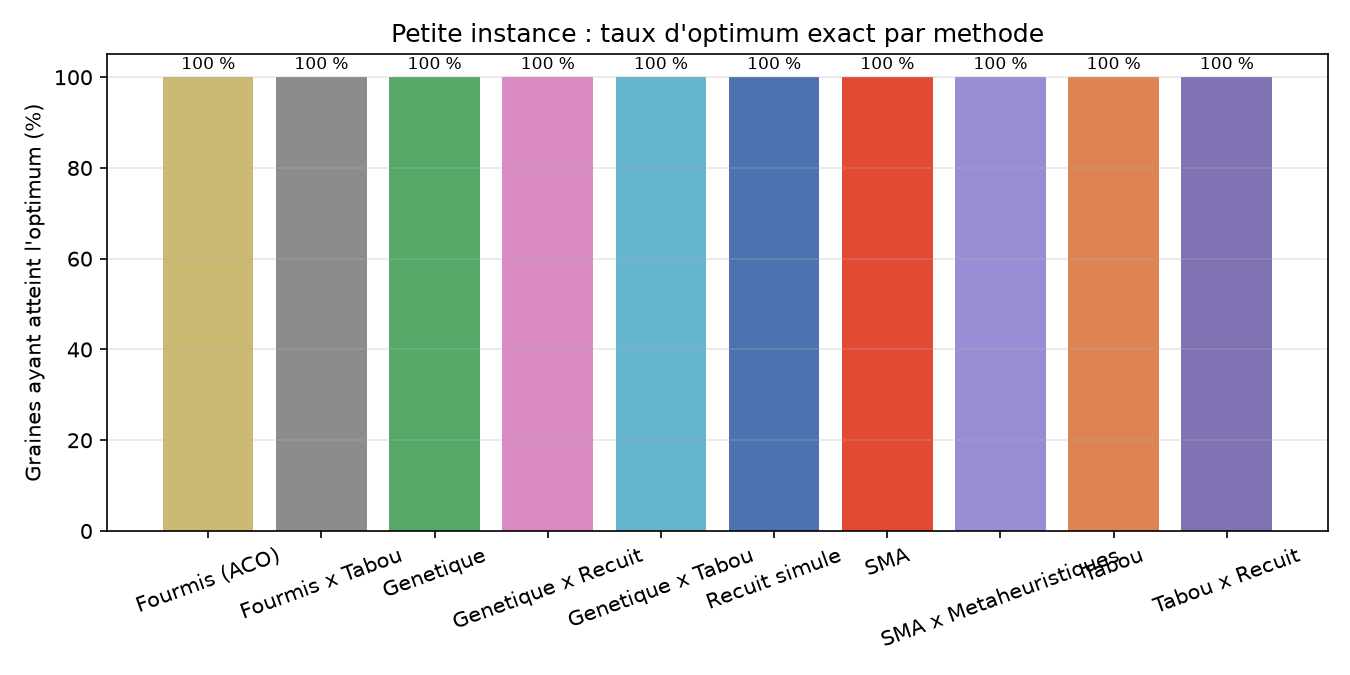
\includegraphics[width=\linewidth,height=0.30\textheight,keepaspectratio]{petite_taux_optimum.png}\\[1pt]
      {\tiny\color{mcmPrimary}\textbf{Petite echelle :}
       10/10 methodes a l'optimum exact (20 graines).}\\[5pt]
      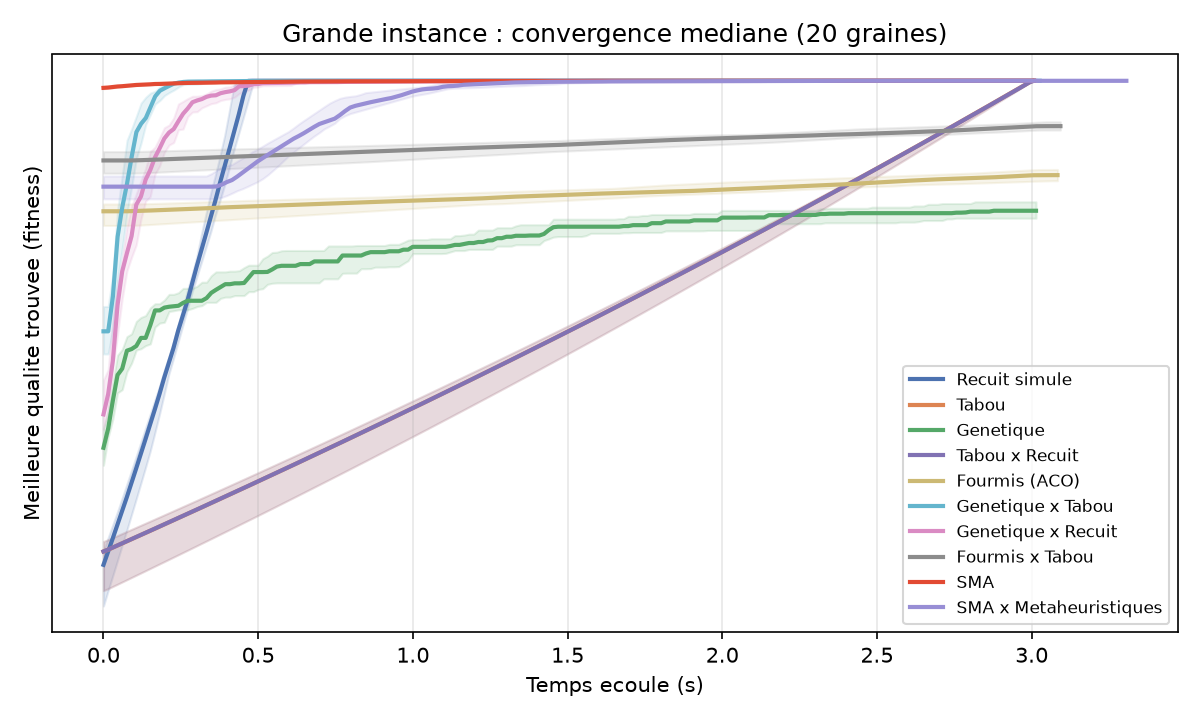
\includegraphics[width=\linewidth,height=0.30\textheight,keepaspectratio]{grande_convergence.png}\\[1pt]
      {\tiny\color{mcmPrimary}\textbf{Grande echelle :}
       convergence a budget egal (300 patients, 3\,s).}
    \end{column}
  \end{columns}
\end{frame}

% Couplage hospital_sim : campagne median/oracle, 1 152 executions.
% Sources : artifacts/full-duration-comparison/{median,oracle}/large/summary.csv
% Filtre : scenario=outage, policy=reactive. Moyennes par taille sur
% 6 methodes x 3 graines x 2 echantillons, soit 36 executions par mode.
% 100 cas : termines 96.2222 / 99.5833 ; depassement 952.8333 / 942.8056 min.
% 300 cas : termines 286.9722 / 300 ; depassement 3104.8333 / 3714.9722 min.
% L'oracle connait les durees d'occupation, mais pas les fermetures futures.


% =============================================================================
% Slide interface : API + application web
% =============================================================================
\begin{frame}[t]{Interface : API et application web}
  \scriptsize
  \begin{center}
    Une API \textbf{FastAPI} et une interface web : inscription et connexion.
  \end{center}
  \vspace{2pt}
  \begin{columns}[T]
    \begin{column}{0.5\textwidth}\centering
      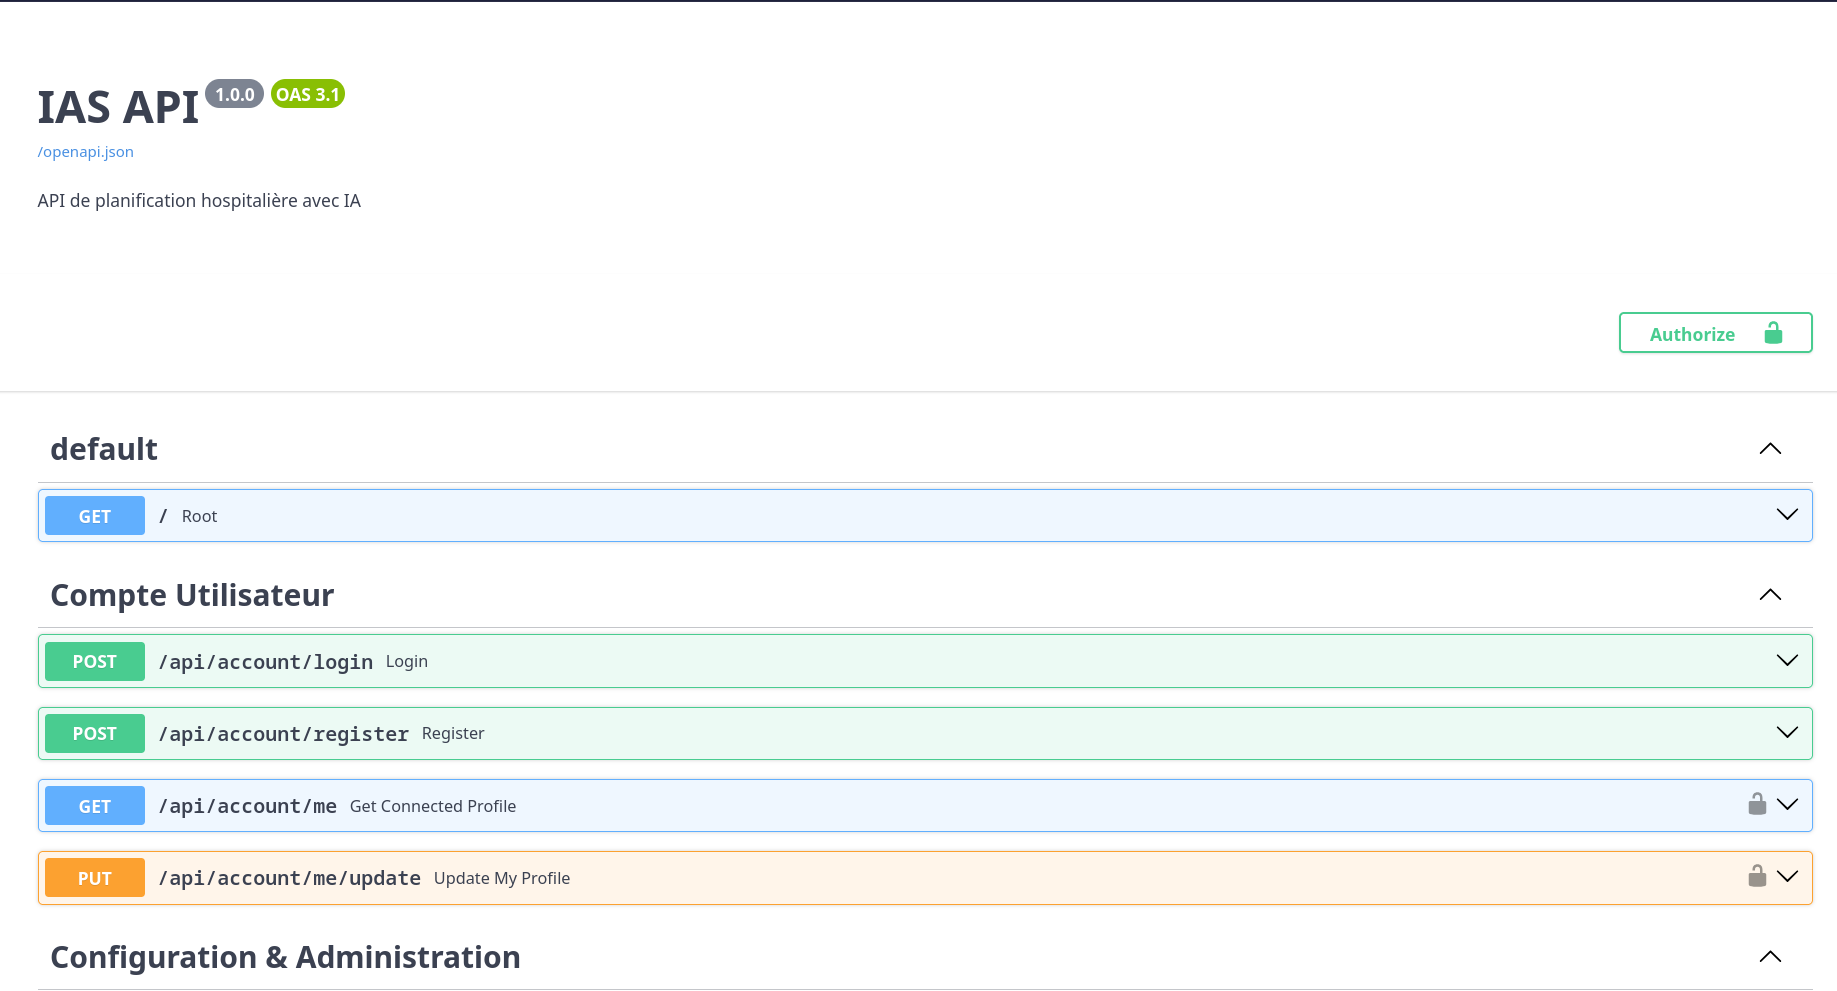
\includegraphics[height=0.40\textheight,keepaspectratio]{screen_API.png}\\[1pt]
      {\tiny API \texttt{IAS API} (Swagger)}
    \end{column}
    \begin{column}{0.25\textwidth}\centering
      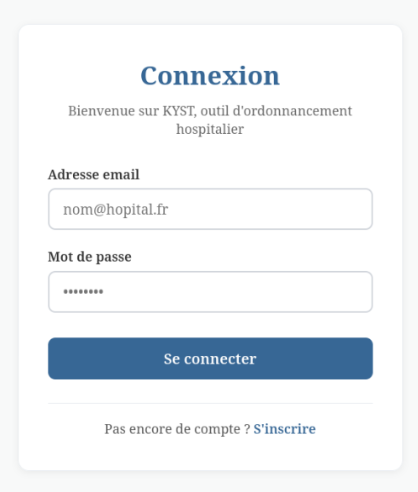
\includegraphics[height=0.40\textheight,keepaspectratio]{capture_interface_connexion.png}\\[1pt]
      {\tiny Connexion}
    \end{column}
    \begin{column}{0.25\textwidth}\centering
      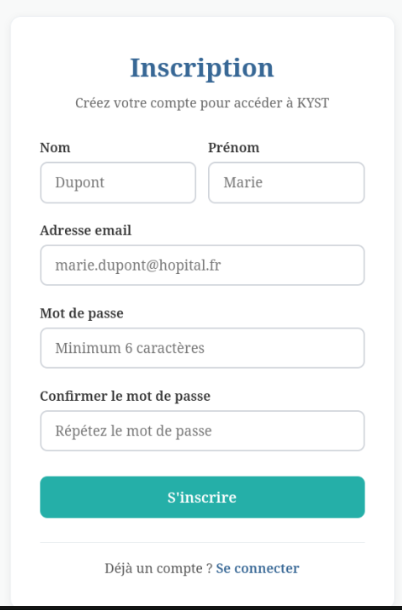
\includegraphics[height=0.40\textheight,keepaspectratio]{capture_interface_inscription.png}\\[1pt]
      {\tiny Inscription}
    \end{column}
  \end{columns}
\end{frame}



\end{document}
